\documentclass[12pt]{report}
%!TeX spellcheck = en_USA

\usepackage{amssymb}
\usepackage{amsmath}

\usepackage{biblatex}
\addbibresource{sample.bib}
\usepackage{titlesec}
\usepackage{float}
\usepackage{graphicx}
\usepackage{amssymb}
\usepackage{titling}
\usepackage[english]{babel}

\usepackage{geometry}
\geometry{
	a4paper,
	total={170mm,257mm},
	left=30mm,
	right=30mm,
	top=30mm,
	bottom=30mm
}

% Title Page
%\renewcommand{\maketitlehookd}{\centering\vfill
\includegraphics{IMGs/Download.jpg}\vfill}

\title{\vspace*{-5cm}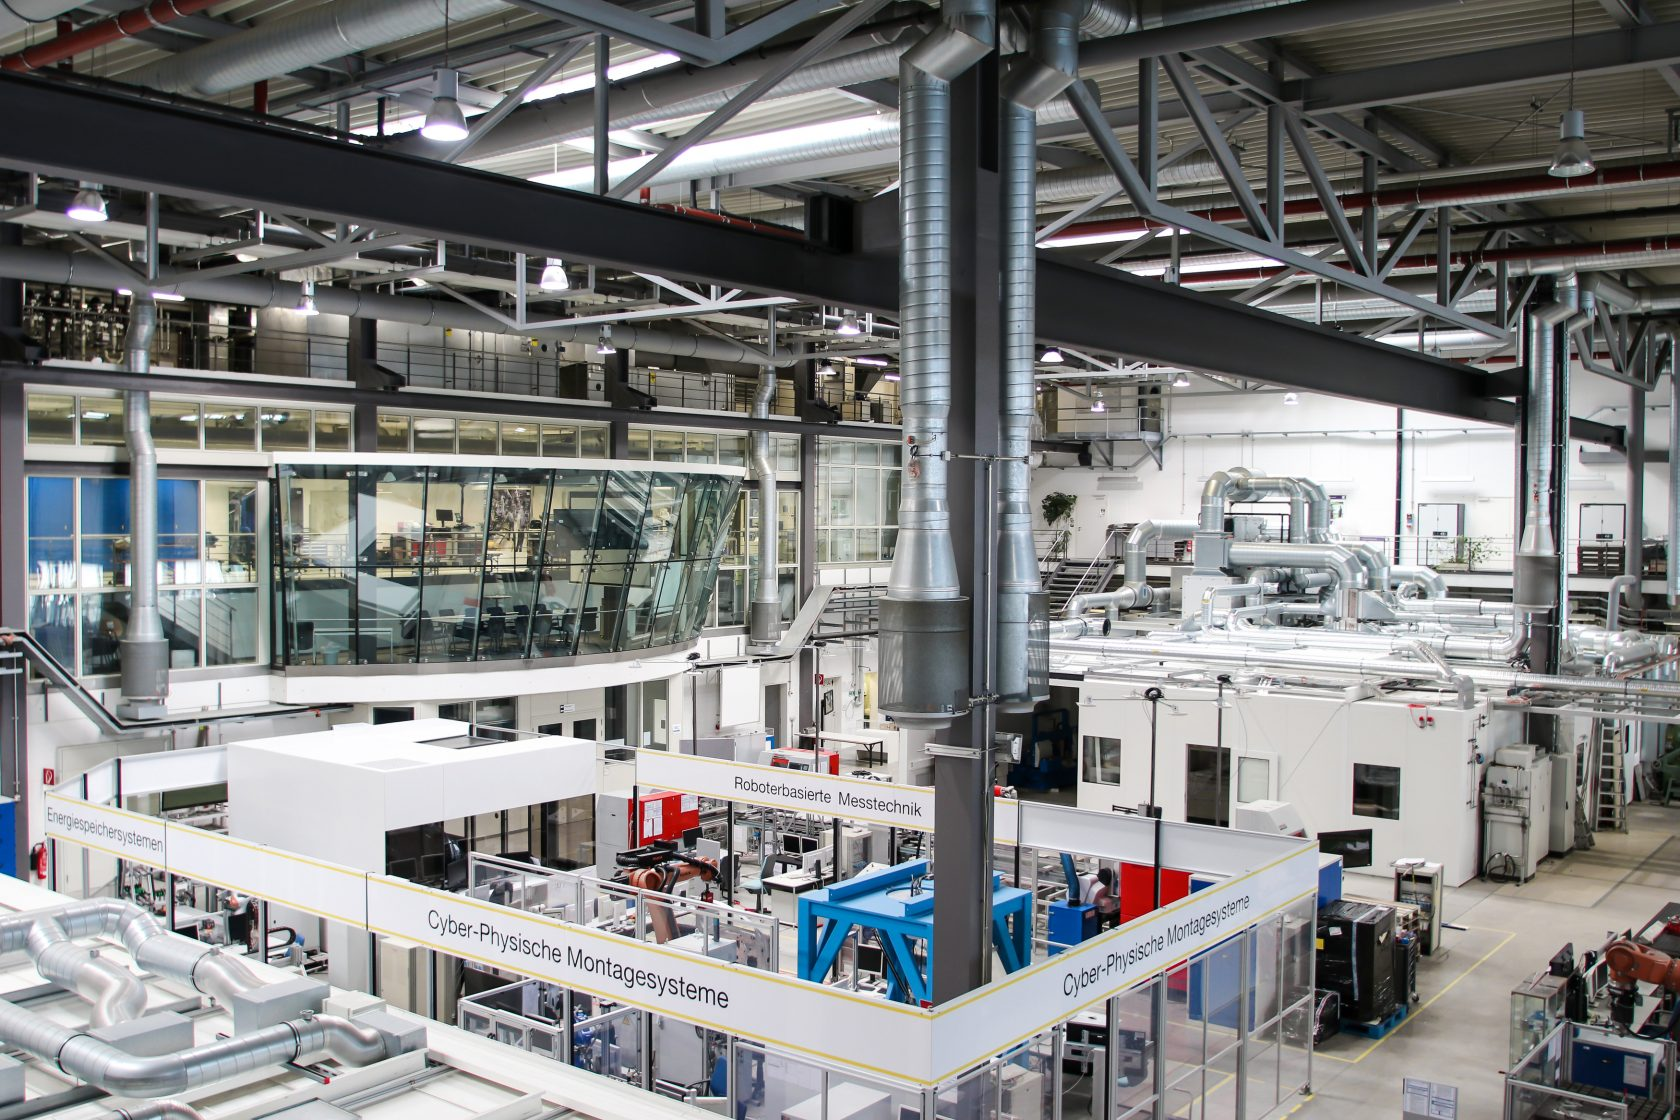
\includegraphics[width=15cm]{../img/deckblatt.jpg}\\Artificial Intelligence in Production Engineering \linebreak \linebreak Group Report \linebreak Group: Predictive Quality Battery}



\author{Nalivaika, Jan\\
	\texttt{03694590}\\
	\texttt{nalivaika@outlook.de}
	\and
	Paździerkiewicz, Przemyslaw\\
	\texttt{03718188}\\
	\texttt{p.pazdzierkiewicz@tum.de}
	\and
	Pielmeier, Sebastian\\
	\texttt{03693728}\\
	\texttt{pielmeier.sebastian@t-online.de}
	\and
	Tcvetkov, Nikita\\
	\texttt{03689859}\\
	\texttt{nikita.tcvetkov@tum.de}
	\and
	Wittner, Simon\\
	\texttt{03696129}\\
	\texttt{simon.wittner@gmx.net}
}


\date{21.07.2022}


%\titleformat{\chapter}[display]   
%{\normalfont\huge\bfseries}{\chaptertitlename\ \thechapter}{20pt}{\Huge}   
%\titlespacing*{\chapter}{0pt}{-60pt}{30pt}


\begin{document}

\maketitle
\begin{abstract}
	Do the other fings first, then compile abstract
\end{abstract}

\tableofcontents
%\renewcommand{\thechapter}{\Roman{chapter}}
\chapter*{List Of Abbreviation}
NN = Neural Net \newline
ML = Machine Learning \newline
FFT = Fast Fourier Transformation\newline
CWT = Continuous Wavelet Transform\newline
STD = Standard Deviation \newline
OOT = out of threshold\newline
RMS = Root mean square\newline
LBW = Lase Beam Welding\newline
KDD = Knowledge Discovery in Databases\newline

\listoffigures

\chapter{Introduction}
%wow das ist soooo cool
%Why is this topic dealt with? Can you motivate your topic by a business case?
%Introducing the reader to the topic
%The reader should understand the general topic and the motivation.

Operating profitably in the current market, requires the capability to adapt to increasingly individualized customer demands, strict adherence to deadlines, and expected quality requirements. Failure to provide the requested services on time or with unacceptable quality deficit will result in a loss of business and lead to being squeezed out of the market.
\newline
In the current state of “Industrie 4.0” and Big-Data, multiple opportunities arise to improve speed and accuracy in the production environment. Adaptive process scheduling, for example, can lead to optimal usage of machinery and adherence to the production schedule. Both of those effects will benefit the costumer, as the product will be manufactured faster and cheaper. When it comes to creating a product for the customer, the production part is only one of the aspects, where the new application possibilities of data-driven algorithms can support the manufacturer. Data-driven algorithms can support the designer to conceptualize more effective mechanisms or help the machinist to react to changing machining parameters, like wear and tear on cutting tools.
Quality control is one of the sections of the production chain where those algorithms can support the identification of rejects or suggest improvements for the production process. The significant advancements in computer science, especially in Machine Learning (ML), can be adapted and transformed to the specific needs of the quality control department, to achieve higher precision rate and efficiency in identifying faults in the final product, than could be done with human labor.
\newline
Machine learning contains those algorithms that are capable of solving tasks without explicitly being programmed to do so. They are based on pattern recognition and their performance improves as more data is available. This property proves them advantageous as more and more data is available from the increasingly digitized production environment. One of the commonly used algorithms in ML are Neural Networks (NNs), which find use in Supervised Learning, Unsupervised Learning and Reinforcement Learning. The main advantage of NNs is that they can be deployed in a multitude of ways, specifically optimized for their intended use cases.
\newpage
This report will provide an exemplary use-case for classifying welds in the domain of laser beam welding. This process can easily be applied to any other classification problem just by adapting a few variables. From a given set of data, multiple preprocessing and feature extraction steps are performed. This procedure follows the general KDD-process (Knowledge Discovery in Databases).
The found features serve as decision bases for the algorithms to classify the welds as “OK” and “not OK”. 


\chapter{Business Case}
In more traditional welding operations, an electric arc is used to bind 2 metallic pieces by selectively melting the material on the two parts and letting it solidify afterwards. One of the disadvantages is that heat-spread during the welding process. Especially with highly conductive materials like copper. This is due to the relatively low power density in electronic arcs. To safely combine 2 materials, it can require a prolonged arc presence, that will heat up the entire parts. When it comes to welding overlapped sheets of material, it can happen that the upper sheet is already molten while the underlying material, due to its high thermal conductivity, is not. Additionally, it requires to have an electric circuit over the two parts to form the arc and start the welding process. This is a disadvantage when it comes to high volume welding operations as it has to be made sure that all connections are stable, and all current is flowing as intended every single time.
The production of battery packs is one of the areas where these disadvantages of arc welding make it very difficult to have a safe and efficient welding process. The welding of the copper conductors to the batteries would require a prolonged heat input that would damage the battery-cells. Additionally, it is not beneficial to expose the batteries to high electrical currents of voltages.


Laser-Beam welding (LBW) is one method that can work with these specific boundary conditions.
The power delivery is very high and leads to an almost instantaneous welding of both materials without conducting a lot of heat to the whole part. Besides that, no electric current is required, which is beneficial for welding battery conductors. By refocusing the beam to the desired position, a high rate of welds per minute can be achieved. As a high weld rate is expected, LBW is one of the favorite methods in battery production.
For validating the welding connection, sensors can record data during the welding process, which can serve as a basis to classify if the desired quality was achieved. %The following sections explain how a set of data has to be analyzed and transformed to be used in the prediction process.

\chapter{Methodology and Experiments}

The Knowledge Discovery in Databases (KDD) process is structured in four steps. At first Data Cleansing is performed to detect data quality issues or remove anomalies. The second step is Data Transformation to select the possible input data. Further, Data Mining is performed to generate to increase the database. Finally, the evaluation is performed to categorieze the success of a model. In teh following sections these steps are perfomed to predict the quality of a weldbeam with the help of a given dataset.


\section{Goal}
The main two objectives are:\newline\newline
1.\newline Determining possible correlations between the measurements of
sensor 1 and 2\newline\newline
2.\newline Classifying the weld seam in four categories (OK , not OK, out of threshold)



\section{Data cleansing and pre-processing}
\subsection{Dataset overview}
As mentioned in the task description, the dataset contains measurements from two different photodiode sensors recording back reflected laser radiation during laser beam welding. Additionally, denoised values for signal one was also given. Each welding seam was divided into five equidistant sections whose measurements were individually recorded as a time series in the dataset. Based on the assignment the welding parameters were assumed to be constant across the dataset.\newline\newline
Each signal log was categorized in four different, equally distributed binary categories: not OK, signal value exceeded, WD40 pollution and Gleitmo pollution. According to the assignment, labeling algorithm first detected if the signal value had been exceeded and if so, the OK/not OK classification was not carried out; thus, in the dataset all samples for which the signal value had been exceeded were uniformly marked as OK. In the second step the data was labeled according to the potentially present lubricant pollution. The labels of the lubricants were found to be exclusive, meaning that for no welding seam both WD40 and Gleitmo were present. In total, 77 (6\%) measurements were identified as “out of threshold”, 996 (74\%) as “OK” and 277 (21\%) as “not OK”. 450 (33\%) weld seams contained no pollution, 450 (33\%) were marked with WD40 and 450 (33\%) with Gleitmo.
\subsection{Data visualization}
Aside from statistical inspection, visualizing the data was the first step in obtaining an overview about features of the dataset. The figures below show plotted signal values for randomly chosen samples with varying labels. As can be seen in figure \ref{fig:VIZ1} and \ref{fig:VIZ2}, attempts were made to reproduce the denoising procedure used for signal 1 for signal 2. Additionally, the automatically calculated Person correlation coefficients between the values for signal 1 and 2 were also displayed.

\begin{figure}[H]
	\centering
	\includegraphics[width=0.9\linewidth]{../img/VIZ1.png}
	\caption{Visualization plot for sample 891}
	\label{fig:VIZ1}
\end{figure}
\begin{figure}[H]
	\centering
	\includegraphics[width=0.9\linewidth]{../img/VIZ2.png}
	\caption{Visualization plot for sample 674}
	\label{fig:VIZ2}
\end{figure}


Based on the data inspection, a few important conclusions could be reached about the dataset: signal 2 was found to be typically much noisier than signal 1 and thus possibly worse for making predictions. Samples marked as “not OK” typically display higher values for all signals; however, no determining boundary distinguishing the two labels could be identified. Furthermore, the correlation coefficients between signals were found to carry little information about the weld quality. Despite reaching the mentioned conclusions, it was difficult to identify the decisive features only based on the visualization. Thus, further analysis including possible data transformation was needed.
\subsection{Data cleansing}
After a careful examination of the dataset an inconsistency regarding the labelling of signals in the “out of threshold” category was identified: multiple samples across the dataset displayed only the value “1” for all signal readings of all the sensors. Although most of such samples were labeled as “out of threshold”, there was a significant number of logs where this was not the case. As the signal values were the only source of input feature for the prediction model, such inconsistency would pose a significant limit to the achieved accuracy. Thus, a new condition for the labeling of the signals was chosen based on the original set of OOT values and the data relabeled accordingly; the new condition being set at 13 occurrences of the value “1” in signal 1 logs, which was the minimum among the samples originally labeled as OOT.

\section{Data Transformation Methodology}
Data Transformation aims at extracting meaningful features from the dataset that can be used for training the classification model. This step is especially important while dealing with often noisy and unstructured time series data, such as provided in the given dataset. There exist many possible approaches to the choice of features and the decision can greatly affect both the learning speed and the output quality of the model. For the given assignment both 1D and 2D transformation techniques were examined, each of them being briefly discussed in the following section. Visualization plots for selected representative samples were also provided for better evaluation of the statistical meaning of each examined feature.
\subsection{Statistical features}
Extracting statistical features allows to transform the dataset of one signal into a single characteristic value that may be decisive about the classification of the signal. In the following section the applied statistical features and the results obtained from the dataset are briefly discussed. For the calculation of each feature, an affiliated method from the pandas, NumPy and SciPy modules were used. Since values obtained from signal 2 were typically noisier and thus yielded worse results for classification compared to signal 1 and signal 1 denoised, only visualizations for the two latter ones were provided.
\subsubsection{Mean}
One of the most prominent statistical approaches is the arithmetic mean. Although in many cases the method is very useful for characterizing the measurement, it also risks filtering out possibly meaningful outliers, which often makes it inadequate for highly varying data. The figures \ref{fig:S1MEAN} and \ref{fig:S1DNMEAN}  below shows the distribution of the mean values of signal one (raw and denoised) across all measurements in the pre-processed dataset with the distinguishment between the OK/NOK labels.

\begin{figure}[H]
	\centering
	\includegraphics[width=0.9\linewidth]{../img/S1_not_OK_MEAN_relabeled.png}
	\caption{The mean values of signal 1 across samples.}
	\label{fig:S1MEAN}
\end{figure}
\begin{figure}[H]
	\centering
	\includegraphics[width=0.9\linewidth]{../img/S1_DN_not_OK_MEAN_relabeled.png}
	\caption{The mean values of denoised signal 1 across samples.}
	\label{fig:S1DNMEAN}
\end{figure}

As seen in the figures \ref{fig:S1MEAN} and \ref{fig:S1DNMEAN} , for both signals the data seems to show a significant correlation between the mean value of the signal and the quality of the weld; poor quality welds tending to correspond to higher mean values. This is especially noticeable across samples affected by pollution with the lubricant Gleitmo (samples 200 through 401 and 950 through 1125). Despite that, there exists a vast region of signals with mean around 0.1 where both OK and NOK samples are found. This confusion region is likely to cause inaccuracies in any classification model using the metric as input which highly undermines its practicality for the model.

\subsubsection{Standard deviation}

Standard deviation (STD) is a popular metric of spread of the values within a sample. Thus, it helps distinguish stable measurements from highly varying ones. In context of quality prediction based on time series data the feature can provide valuable information about possible changes detected in the weld seam. The figure below shows the distribution of standard deviation values across the dataset.

\begin{figure}[H]
	\centering
	\includegraphics[width=0.9\linewidth]{../img/S1_not_OK_STD_relabeled.png}
	\caption{The Standard deviation of signal 1 across samples.}
	\label{fig:S1STD}
\end{figure}
\begin{figure}[H]
	\centering
	\includegraphics[width=0.9\linewidth]{../img/S1_DN_not_OK_STD_relabeled.png}
	\caption{The Standard deviation of denoised signal 1 across samples.}
	\label{fig:S1DNSTD}
\end{figure}

Based on the plot (see figures \ref{fig:S1STD} and \ref{fig:S1DNSTD}) the signal’s standard deviation seems slightly more adequate for OK/NOK classification of the samples than the mean; the boundary between the two clusters being more protruding. The effect is again augmented by the presence of Gleitmo lubricant. However, the confusion region in this case is still very prominent which again questions the metric’s applicableness.

\subsubsection{Minimum, maximum and percentiles}
Other easily identifiable characteristic features within a sample are the maximum, the minimum, as well as the value at a given percentile (most commonly used being Q25, Q75, and Q50 aka the median). The plot below shows the scattering of the first signal’s maximal value across samples which proved to be the most significant metric across all the others mentioned in this section.

\begin{figure}[H]
	\centering
	\includegraphics[width=0.9\linewidth]{../img/S1_not_OK_MAX_relabeled.png}
	\caption{The maximum values of signal 1 across samples.}
	\label{fig:S1MAX}
\end{figure}
\begin{figure}[H]
	\centering
	\includegraphics[width=0.9\linewidth]{../img/S1_DN_not_OK_MAX_relabeled.png}
	\caption{The maximum values of denoised signal 1 across samples.}
	\label{fig:S1DNMAX}
\end{figure}
Based on the visualization the maximal value seems to be the most promising feature for OK/NOK classification compared to the other examined ones. Nevertheless, a significant confusion region is still noticeable. This is likely due to the metric’s sensitivity to sudden changes which the signals exhibit.

\subsubsection{Root mean square}
The Root mean square (RMS) of a sample is defined as the square root of the arithmetic mean of the squared values in the sample. It is widely used in signal processing as it can be interpreted as the strength of the signal. The plots below show the spreading of the RMS values for signal 1 across samples.
\begin{figure}[H]
	\centering
	\includegraphics[width=0.9\linewidth]{../img/S1_not_OK_RMS_relabeled.png}
	\caption{The RMS values of signal 1 across samples.}
	\label{fig:S1RMS}
\end{figure}
\begin{figure}[H]
	\centering
	\includegraphics[width=0.9\linewidth]{../img/S1_DN_not_OK_RMS_relabeled.png}
	\caption{The RMS values of denoised signal 1 across samples.}
	\label{fig:S1DNRMS}
\end{figure}
As can be seen on figures \ref{fig:S1RMS} and \ref{fig:S1DNRMS} the RMS shows a similar pattern as the already examined mean and STD; faulty samples typically exhibiting a higher value, which is still augmented by the presence of a lubricant, especially Gleitmo. Again, based on the visualization a quite significant confusion region can be seen as well.

\subsubsection{Skewness}
Skewness is a measure of the asymmetry of the probability distribution of a real-valued random variable around its mean value. For positive skewness more samples have a height value smaller than the mean; the opposite being true for negatively skew distribution (1). The plots below show the distributions of sample skewness for signal 1 and signal 1 denoised across the measurements.
\begin{figure}[H]
	\centering
	\includegraphics[width=0.9\linewidth]{../img/S1_not_OK_Skewness_relabeled.png}
	\caption{The Skewness of signal 1 across samples.}
	\label{fig:S1SK}
\end{figure}
\begin{figure}[H]
	\centering
	\includegraphics[width=0.9\linewidth]{../img/S1_DN_not_OK_Skewness_relabeled.png}
	\caption{The Skewness of denoised signal 1 across samples.}
	\label{fig:S1DNSK}
\end{figure}

As visible in the graphs, the poor differentiation of skewness values between the labels for both signals make the feature unsuitable for the classification task. It suggests that there is hardly any correlation between the weld quality and the proportions of the signal’s distribution.
\subsubsection{Entropy}
Entropy is another statistical feature often applied for time series data. It is the measure of impurity associated with a random variable. A sample containing more noise will have a higher entropy value. The graph below shows the distribution of entropy values for signal 1 across the dataset.
\begin{figure}[H]
	\centering
	\includegraphics[width=0.9\linewidth]{../img/S1_not_OK_Entropy_relabeled.png}
	\caption{The Entropy of signal 1 across samples.}
	\label{fig:S1EN}
\end{figure}
\begin{figure}[H]
	\centering
	\includegraphics[width=0.9\linewidth]{../img/S1_DN_not_OK_Entropy_relabeled.png}
	\caption{The Entropy of denoised signal 1 across samples.}
	\label{fig:S1DNEN}
\end{figure}
Based on the graph for the denoised data yet again a characteristic pattern can be seen for samples of both categories; the NOK measurements having typically lower entropy values. Still, it is difficult to identify an unambiguous boundary between the two clusters which makes the metric unsuitable for effective classification. For the raw signal data the points are even more indistinguishable from each other. This is likely caused by the large amount of noise in the measurements.

\section{FFT}
FFT or Fast Fourier Transform is an algorithm to transform a signal from time-space domain into frequency domain. It’s often used to analyze stationary systems and its vibrations. (cite:Signalverarbeitung) In our research we did perform a FFT with a hope to reveal some more information out of data during feature engineering process. 




To transform the signal python scipy.fftpack package with default parameters was used to perform the FFT transformation. At first signal 1 and Signal 1 DN were transformed for Sample 2 and plotted. Figure \ref{fig:FFT1} shows these 2 Signals after transformation. Signal 1 DN has 1 peak at 0 and is constant showing no peaks (no further information). Signal 1 has multiple peaks all over the spectrum. Therefore, we will take signal 1 as input for further FFT analysis.

\begin{figure}[H]
	\centering
	\includegraphics[width=\linewidth]{../img/FFT1.png}
	\caption{FFT1}
	\label{fig:FFT1}
\end{figure}

In figure \ref{fig:FFT2} and \ref{fig:FFT3} of signal 1 for the four samples are shown. On the left plot Sample 3 is shown which was contaminated with WD 40 has an NOK = 0 label while Sample 203 was contaminated with Gleitmo is NOK = 1. While observing the two FFT’s from 2 different samples no obvious differences can be registered. Both samples have a peak at frequency = 0 which can be interpretated as a vibration with a very big period. In comparison to the left plot, on the right both samples are NOK = 0. Similarly to the plot on the left no huge differences can be detected between these two samples. Thus, it can be said, FFT doesn’t reveal the difference between:


1)	NOK or OK


2)	WD40 or Gleitmo\newline
And isn’t useful as an input for the classifier.

\begin{figure}[H]
	\centering
	\includegraphics[width=\linewidth]{../img/FFT2.png}
	\caption{FFT2}
	\label{fig:FFT2}
\end{figure}
\begin{figure}[H]
	\centering
	\includegraphics[width=\linewidth]{../img/FFT3.png}
	\caption{FFT3}
	\label{fig:FFT3}
\end{figure}


\section{Continuous Wavelet Transformation}
Similarly to Fourier Transform, the wavelet transform maps the signal from time to frequency domain; the key difference being that is also provides time resolution of the transformed signal which makes it more suitable for analyzing non-stationary systems (3). The reasoning behind applying CWT upon the provided dataset was the assumption that certain changes in the signal’s frequency may be caused by particular defects in the welding seam. Furthermore, a wavelet-based algorithm was also mentioned as a part of the labelling process which suggested that the transform may yield valuable information about the weld seam quality.
The transform was carried out with help of the pywavelets module using the Morlet wavelet and varying ranges of scaling factors (up to 1000). The transformed data was subsequently visualized with the intention of identifying any possible underlying patterns. The following figures show exemplary plots for two randomly chosen samples with differing labels.
\begin{figure}[H]
	\centering
	\includegraphics[width=0.9\linewidth]{../img/Sample_283_DN_(OK).png}
	\caption{CWT visualization for sample 283 (Signal 1 denoised).}
	\label{fig:CWT1}
\end{figure}
\begin{figure}[H]
	\centering
	\includegraphics[width=0.9\linewidth]{../img/Sample_984_DN_(NOK).png}
	\caption{CWT visualization for sample 984 (Signal 1 denoised).}
	\label{fig:CW2}
\end{figure}
As demonstrated by the above figures, no compelling correlation between the labelling and the wavelet transform coefficients of the signal could be identified. Thus, it was decided not to include the transformed data in further consideration. It is possible that the seemingly poor performance of the approach resulted from the inappropriate choice of the transform parameters. However, their adjustment would require additional knowledge about the data collection and labelling process which was not provided.


\section{Classification Models} 
In accordance with the KDD process, different models for finding patterns in the pre-processed data are considered.  The three different models presented in the following chapters are chosen based on previous publications regarding predictive quality classification in production engineering and recent trends in machine learning.
%NN
%LOG REG
%LS
%baeysian regression
%Gradientren Boosting
\subsection{LOG REG}
Logistic Regression is a method of binary classification (2 classes). It is mostly used In statistics and made its way to machine learning. The method called so after the logistic function (sigmoid function) which maps any real value in value between 0 and 1. (https://machinelearningmastery.com/logistic-regression-for-machine-learning/)
This output is equivalent to the predicted probability P\_i of the input X\_i belonging to the class y\_i  (falls platz hier die gleichung). 
The final discrete classification is based on the whether the probability P\_i is great or equal/smaller than 0.5.




\subsection{Gradient boosting}
Gradient boosting is a recent machine learning technique used for regression and classification tasks based on ensemble learning. Many weak prediction models are averaged and result in a strong prediction model. XGBoost is a gradient boosting method based on decision trees. It has gained popularity because of its very good performance in machine learning competitions  . XGBoost also impresses with its high computing speed.\cite{ What is XGBoost? | Data Science | NVIDIA Glossary, XGBoost | Kaggle}
The hyperparameters of the “XGBoost” gradient boosting model are:
-	The number of iterations in the model generation cycle
-	The learning rate/the weight of each model for the final prediction
Considering the limited computational resources at hand they are optimized using a randomized non-exhaustive grid search. For the final model the number of model generation cyles is set to XXXX and the learning rate to XXXX.
Furthermore, we performed a principal component analysis to improve in calculation speed and complexity.





\subsection{Usage of a Neural Network}



Another kind of model which can be used for the classification of data are Neural Networks (NNs). They consist of an input layer, multiple hidden layers and an output layer. The number of neurons in the hidden layers is arbitrary while in the input and output layer it corresponds with the dimension of the input/output. Depending on the task of the neural network (Regression or Classification), the so-called activation function in the output layers is chosen. The activation function determines the mathematical operations performed at each node. For the hidden layers the choice of the activation function is independent of the application of the NN.
For a NN, a large number of hyperparameters must be determined. The main ones are:\newline\newline
-	Optimizer and Learning rate\newline\newline
-	Activation function\newline
-	Architecture of the NN (number of hidden layers and respective number of neurons)\newline
Based on engineering practices presented in the courses “AI in Production Engineering” and “Physics-informed machine learning”, as well as the paper “Real-time prediction of…”, the widely used ADAM optimizer is chosen together with a learning rate of 0.001. 
Since a binary classification must be conducted, the “Sigmoid” activation function is used in the output layer.
For the activation functions of the hidden layers, the hyperbolic tangent (tanh) and the Rectified Linear Unit (ReLu) function are considered. Their performance with different NN architectures (1-7 layers, 5 – 100 neurons) is evaluated in multiple tests using a cross validation. The results show that especially with bigger NNs, a higher mean prediction accuracy can be achieved using the ReLu function. However, this comes at the expense of a higher variance and a gradual decrease in the share of false negatives/a gradual increase in the share of false positives. This indicates at least a partial overfit of the model on the dataset. Considering the planned application of the model, an emphasis is put on the robustness of the expected prediction and the prevention of a bias due to overfitting. Therefore, a model architecture with only one hidden layer and 75 neurons, using the tanh activation function is chosen.  




Another kind of model which can be used for the classification of data are Neural Networks (NNs), also referred to as Multilayer Perceptrons. They are composed of an input layer, multiple hidden layers and an output layer. The number of neurons, also called nodes, in the hidden layers is arbitrary while in the input and output layer it corresponds with the dimension of the input/output. Depending on the task of the neural network (Regression or Classification), the so-called activation function in the output layers is chosen. The activation function determines the mathematical operations performed at each node. For the hidden layers the choice of the activation function is independent of the application of the NN.
The main advantages of Neural Networks are their universality, which is a result of the nonlinearities in the neurons and their ability to efficiently approximate functions in high-dimensional spaces. These properties are especially useful when considering complex datasets.
For a NN, a large number of hyperparameters must be determined. The main ones are:\newline\newline
-	Architecture of the NN (number of hidden layers and respective number of neurons)\newline
-	Activation function\newline
-	Optimizer and Learning rate\newline\newline



\chapter{Results}
In the following chapter the performance of the three different classification models is evaluated. For this comparison the accuracy metric (share of correct predictions) and its spread are considered, as well as the share of false positives and false negatives.
Intercomparability between the results of the different models is ensured by using the same ten-fold stratified cross validation for all input/output combinations and models.
All the results are obtained using the denoised data from sensor 1. The predictions with this data set proved to be continuously superior or equal to the ones obtained using the other data sets (maybe cite data chapter with plots). 
Additionally, all samples considered to be incorrectly classified as “within signal threshold” are removed in accordance with the procedure described in chapter X.X.


\section{results LOG}
At first, data was read. For the input label–columns were dropped from the data-table, so just all 112 Signal values represented the input. Input was assigned to X and label-column to y. Which labels were used depended upon in which classes the classification were to conduct. So for example for the OK/NOK classification the NOK column was assigned to y. 
\newline
Afterwards train/test split was conducted. The typical 70/30 split ratio was used. Random state wasn’t engaged. The logistic regression model was created with pythons library “sklearn” and its class “Pipeline”. max\_iter = 1e5 parameter was given.\newline



The model performed best on the RAW data input. Signal 1 performed the same as the signal 1\_dn. The results are shown in the figure. The accuracies were obtained with Signal 1\_dn as input.
\begin{figure}[H]
	\centering
	\includegraphics[width=\linewidth]{../img/log.png}
	\caption{Results of Logistic Regression. Y = Classification 
		X = Input 
	}
	\label{fig:log}
\end{figure}





\section{resulots gradientr boost }
We use the XGBoost library for predicting the quality of battery contacting and to compare the performance to the other used models (neural network and logistic regression). In a first step, we preprocessed our data. Our features are represented by each 112 signal values from 2 sensors as input and our label consists of the respective classification goal. Data from sensor 1 was already denoised. We used wavelets to denoise the signals from sensor 2 in MATLAB. We then conducted a train-test split with the typical split ratio of 70/30 to train the model. For better comparability of our models, to avoid overfitting and to get the best indicator for our overall performance, we performed a stratified cross validation with 10 folds. In order to improve our hyperparameters and the result, a randomized (not exhaustive) grid search was conducted. Furthermore, we performed a principal component analysis to improve in calculation speed and complexity. Table 1 shows our results for the different classification tasks and our best performing feature combinations. “Sensor 1dn” are the denoised signals from sensor 1. “Sensor 2MAT” are the manually denoised signals with MATLAB from sensor 2.

\begin{figure}[H]
	\centering
	\includegraphics[width=\linewidth]{../img/GB.png}
	\caption{Results of Gradient boosting with different features
	}
	\label{fig:GB}
\end{figure}

Since we only have limited calculation resources, we performed a not exhaustive grid search for hyperparameter optimization. In order to obtain the best results, it would be beneficial to perform an exhaustive grid search in a next step. The performance of our estimator would also benefit from further feature engineering approaches and more train data. 

\section{Results of the NN}


The test results show that especially with bigger NNs, a higher mean prediction accuracy can be achieved using ReLu (approx. 93\%), while the accuracy of the networks using the tanh function reaches its maximum accuracy of around 91\% already with two hidden layers and then stagnates.
The variance of the prediction accuracy ranges between approx. 1.2\% and approx. 4.1\%. In average, it is around 1\% higher when using ReLu.
For the NN architectures using only one hidden layer, the shares of false positives and false negatives are similar (approx. 5.8\% vs approx. 4.8\%). However, already with three hidden layers, the share of false negatives decreases to around 2.8\%, while the share of false positives increases to around 6.2\%. Especially with higher numbers of hidden layers this effect is more pronounced when using the ReLu activation function. This indicates at least a partial overfit of the model on the dataset.
Considering the planned application of the model, an emphasis is put on the robustness and reliability of the expected prediction. Therefore, a model architecture with only one hidden layer and 75 neurons, using the tanh activation function is chosen. The expected prediction accuracy is 89\%, which is around four percent lower than the results obtained with more complex models. However, the expected very low variance of the results (1.33\%) and the balance between the shares of false negatives and false positives (6.1\% vs 4.9\%) ensure the reliability of the prediction and minimize the risk of possible overfitting. Especially in production engineering, a bias in the predictions introduced by overfitting can have detrimental effects on the practical usability of a model and may nullify its practical use in the long term.

Figure \ref{fig:NN} shows the prediction accuracy for different labels y using the NN with the hyperparameters described in X.X. All predictions were done using the raw, but denoised data of sensor 1 or derived statistical metrics as the input of the NN as this gave the highest accuracies, regardless of the data label.
It is not possible to correctly predict for the label ‘WD40’ and ‘Lubricant’. In both cases the NN classifies all outputs the same. This problem persists, regardless of the input.
The predictions for the label ‘Gleitmo’ are slightly better, albeit also with a strong tendency for false negatives. 
In summary, correctly predicting the presence or the kind of lubricant at the weld seam is not possible with the available data sets and used statistical metrics.

\begin{figure}[H]
	\centering
	\includegraphics[width=\linewidth]{../img/NN.png}
	\caption{Results of the classification using a NN}
	\label{fig:NN}
\end{figure}

\subsection{Classification of sample quality (OK, Not OK) }
Table X.X shows the mean prediction accuracy and the standard deviation of the prediction accuracy of the three different classification methods for the weld-seam quality label (Ok, Not Ok). Apart from the raw data, different statistical metrics are considered as input features. The hyperparameters are set according to chapter X.X.
Regardless of the input, high mean prediction accuracies above 82\% are achieved. Additionally, the calculated standard deviations are low (< 2.5\%). In contrast to the other methods, the prediction accuracy of the NN improves when using the derived statistical metrics as input. 


\begin{figure}[H]
	\centering
	\includegraphics[width=\linewidth]{../img/S1.png}
	\caption{Results for the weld-seam quality label (Ok, Not Ok)}
	\label{fig:S1}
\end{figure}

The shares of the false positives (parts incorrectly classified as “OK”) and false negatives (parts incorrectly classified as “Not OK”) are shown in table X.X. All methods exhibit a bias towards incorrectly classifying samples as “Not OK”. This phenomenon is most prevalent for the predictions using the statistical metrics as an input and especially for the Logistic Regression and Gradient boosting methods.

\begin{figure}[H]
	\centering
	\includegraphics[width=\linewidth]{../img/S2.png}
	\caption{Bias towards incorrectly classifying samples}
	\label{fig:S2}
\end{figure}

\subsection{Classification of lubricant (WD40, Gleitmo, no lubricant)} 
The results for the prediction accuracy of the presence of WD40 lubricant at the weld seam are presented in table X.X. Regardless of the model and the input data, all evaluated metrics (mean prediction accuracy, standard deviation of the prediction, share of false positives and negatives) remain unchanged. The reason for this outcome is that all inputs are assigned to the same class (“No WD40 present”).
The inverse case is observed when trying to predict the presence of lubricant, not considering its exact designation. Here, all inputs are assigned to the class “Lubricant present”, again regardless of the input (mean prediction accuracy: 64.79\%, standard deviation of the results: 0.29).
The predictions for the presence of Gleitmo are slightly better when using a NN (mean prediction accuracy: > 71\%, standard deviation of the results:  < 3.14), albeit also with a distinct tendency for false negatives (share of false positives > 2.17\%, share of false negatives < 26.45\%)

\begin{figure}[H]
	\centering
	\includegraphics[width=\linewidth]{../img/S3.png}
	\caption{Prediction accuracy of the presence of WD40 lubricant at the weld seam }
	\label{fig:S3}
\end{figure} 

\begin{figure}[H]
	\centering
	\includegraphics[width=\linewidth]{../img/S4.png}
	\caption{predictions for the presence of Gleitmo }
	\label{fig:S4}
\end{figure}


\chapter{Discussion}
Confusion Matrix
unterscheidung von Gleitmittel?

What are levers to increase the model performance? Is hyper-parameter tuning possible and
sensible? Is your model sensitive to random seeds and train/test-splits?
How robust is the model when reducing the number of training observa-
tions?

Core of the report???
Interpretation and evaluation of the results
Direct references to the results of the previous section

How can the results be interpreted, what are the consequences and
limitations?


\chapter{Summary and Outlook}
If you had more time, what would your next steps be? How applicable
is your model in real-world use cases?

Indicate the key findings you had and the future research you would
conduct if you had more time

\chapter{Appendix}
\printbibliography
%\renewcommand{\thechapter}{\Roman{chapter}}
%\setcounter{chapter}{2}
\chapter{Contents of the project folder}

\end{document}          
